\documentclass[tikz,border=4pt]{standalone}
\begin{document}
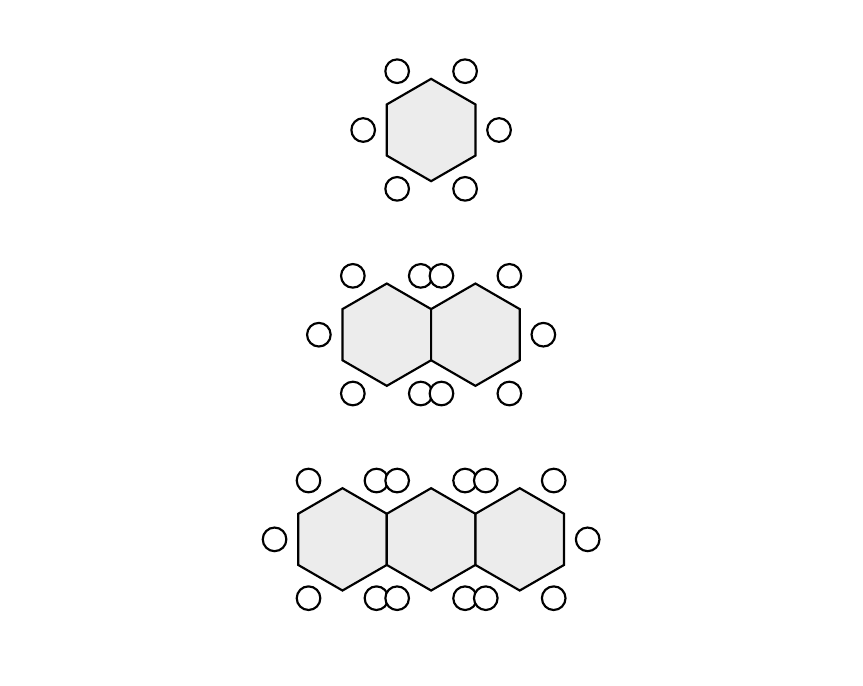
\begin{tikzpicture}[x=0.025cm,y=-0.025cm]
\path[use as bounding box] (0,0) rectangle (410,320);
\path[fill=gray!15,draw=black,line width=0.78pt] (205,26) -- (227.517,39) -- (227.517,65) -- (205,78) -- (182.483,65) -- (182.483,39) -- cycle;
\path[fill=white,draw=black,line width=0.78pt] (222.258,22.108) circle[radius=6];
\path[fill=white,draw=black,line width=0.78pt] (239.517,52) circle[radius=6];
\path[fill=white,draw=black,line width=0.78pt] (222.258,81.892) circle[radius=6];
\path[fill=white,draw=black,line width=0.78pt] (187.742,81.892) circle[radius=6];
\path[fill=white,draw=black,line width=0.78pt] (170.483,52) circle[radius=6];
\path[fill=white,draw=black,line width=0.78pt] (187.742,22.108) circle[radius=6];
\path[fill=gray!15,draw=black,line width=0.78pt] (182.483,130) -- (205,143) -- (205,169) -- (182.483,182) -- (159.967,169) -- (159.967,143) -- cycle;
\path[fill=white,draw=black,line width=0.78pt] (199.742,126.108) circle[radius=6];
\path[fill=white,draw=black,line width=0.78pt] (199.742,185.892) circle[radius=6];
\path[fill=white,draw=black,line width=0.78pt] (165.225,185.892) circle[radius=6];
\path[fill=white,draw=black,line width=0.78pt] (147.967,156) circle[radius=6];
\path[fill=white,draw=black,line width=0.78pt] (165.225,126.108) circle[radius=6];
\path[fill=gray!15,draw=black,line width=0.78pt] (227.517,130) -- (250.033,143) -- (250.033,169) -- (227.517,182) -- (205,169) -- (205,143) -- cycle;
\path[fill=white,draw=black,line width=0.78pt] (244.775,126.108) circle[radius=6];
\path[fill=white,draw=black,line width=0.78pt] (262.033,156) circle[radius=6];
\path[fill=white,draw=black,line width=0.78pt] (244.775,185.892) circle[radius=6];
\path[fill=white,draw=black,line width=0.78pt] (210.258,185.892) circle[radius=6];
\path[fill=white,draw=black,line width=0.78pt] (210.258,126.108) circle[radius=6];
\path[fill=gray!15,draw=black,line width=0.78pt] (159.967,234) -- (182.483,247) -- (182.483,273) -- (159.967,286) -- (137.45,273) -- (137.45,247) -- cycle;
\path[fill=white,draw=black,line width=0.78pt] (177.225,230.108) circle[radius=6];
\path[fill=white,draw=black,line width=0.78pt] (177.225,289.892) circle[radius=6];
\path[fill=white,draw=black,line width=0.78pt] (142.708,289.892) circle[radius=6];
\path[fill=white,draw=black,line width=0.78pt] (125.45,260) circle[radius=6];
\path[fill=white,draw=black,line width=0.78pt] (142.708,230.108) circle[radius=6];
\path[fill=gray!15,draw=black,line width=0.78pt] (205,234) -- (227.517,247) -- (227.517,273) -- (205,286) -- (182.483,273) -- (182.483,247) -- cycle;
\path[fill=white,draw=black,line width=0.78pt] (222.258,230.108) circle[radius=6];
\path[fill=white,draw=black,line width=0.78pt] (222.258,289.892) circle[radius=6];
\path[fill=white,draw=black,line width=0.78pt] (187.742,289.892) circle[radius=6];
\path[fill=white,draw=black,line width=0.78pt] (187.742,230.108) circle[radius=6];
\path[fill=gray!15,draw=black,line width=0.78pt] (250.033,234) -- (272.55,247) -- (272.55,273) -- (250.033,286) -- (227.517,273) -- (227.517,247) -- cycle;
\path[fill=white,draw=black,line width=0.78pt] (267.292,230.108) circle[radius=6];
\path[fill=white,draw=black,line width=0.78pt] (284.55,260) circle[radius=6];
\path[fill=white,draw=black,line width=0.78pt] (267.292,289.892) circle[radius=6];
\path[fill=white,draw=black,line width=0.78pt] (232.775,289.892) circle[radius=6];
\path[fill=white,draw=black,line width=0.78pt] (232.775,230.108) circle[radius=6];
\end{tikzpicture}
\end{document}
